\chapter{ANÁLISE DOS RESULTADOS}\label{ch:conclusao}

Este capítulo tem como finalidade apresentar os resultados obtidos através das implementações demonstrados no Capítulo~\ref{ch:implementacao}.

\section{APRESENTAÇÃO DOS RESULTADOS}

Após o mapeamento das informações do \textit{DataFrame}, apresentado pelo Código~\ref{ini-py} e Código~\ref{map-lingua}, foi construído um gráfico em barras indicando as quantidades de \textit{tweets} em relação aos quatro idiomas mais significativos no conjunto de dados coletados, Gráfico~\ref{lingua}.

\begin{grafico}[h!]
	\centering
	\fbox{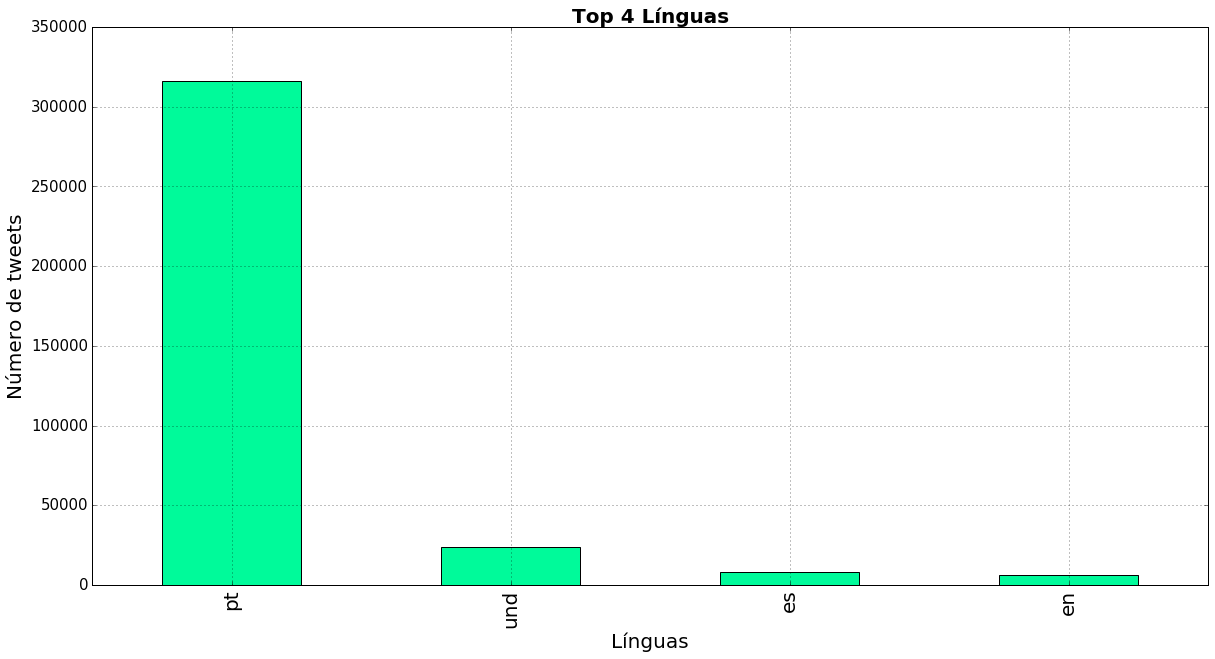
\includegraphics[width=1\textwidth]{Cap6/graficos/linguas}}
	\vspace{-0.2cm}
	\caption{Idiomas que mais realizaram \textit{tweets}}
	\fonte{Elaborado pelo autor}
	\label{lingua}
\end{grafico}

É possível verificar nesta figura que existe uma barra com o nome de \textit{und} para especificar o segundo idioma que mais realizou \textit{tweets}. Essa é uma condição em que não foi identificado o idioma de origem e, então, a API do \textit{Twitter} classifica como \textit{undefined}, ou indefinido no português. Essa linguagem indefinida ocorre devido ao \textit{software} em que o usuário está realizando o \textit{tweet}, por exemplo; um navegador \textit{web}, um aplicativo \textit{mobile} do \textit{Twitter} ou algum aplicativo de terceiro que permite realizar ações no \textit{Twitter}. Caso a linguagem não esteja definida nestes ambientes, a API a classifica como indefinida \cite{twitter-doc}.

O Gráfico~\ref{paises} demonstra, claramente, que a maior número de \textit{tweets} foram publicados do Brasil e apenas uma pequena quantia deles foram realizados nos Estados Unidos, Argentina, Portugal e Venezuela. É importante notar que nem todos os \textit{tweets} gerados possuem um país de origem, o que se assemelha a situação anterior, onde a API do \textit{Twitter} os classifica como \textit{undefined}, porém não sendo apresentado no Gráfico~\ref{paises}.

\begin{grafico}[h]
	\centering
	\fbox{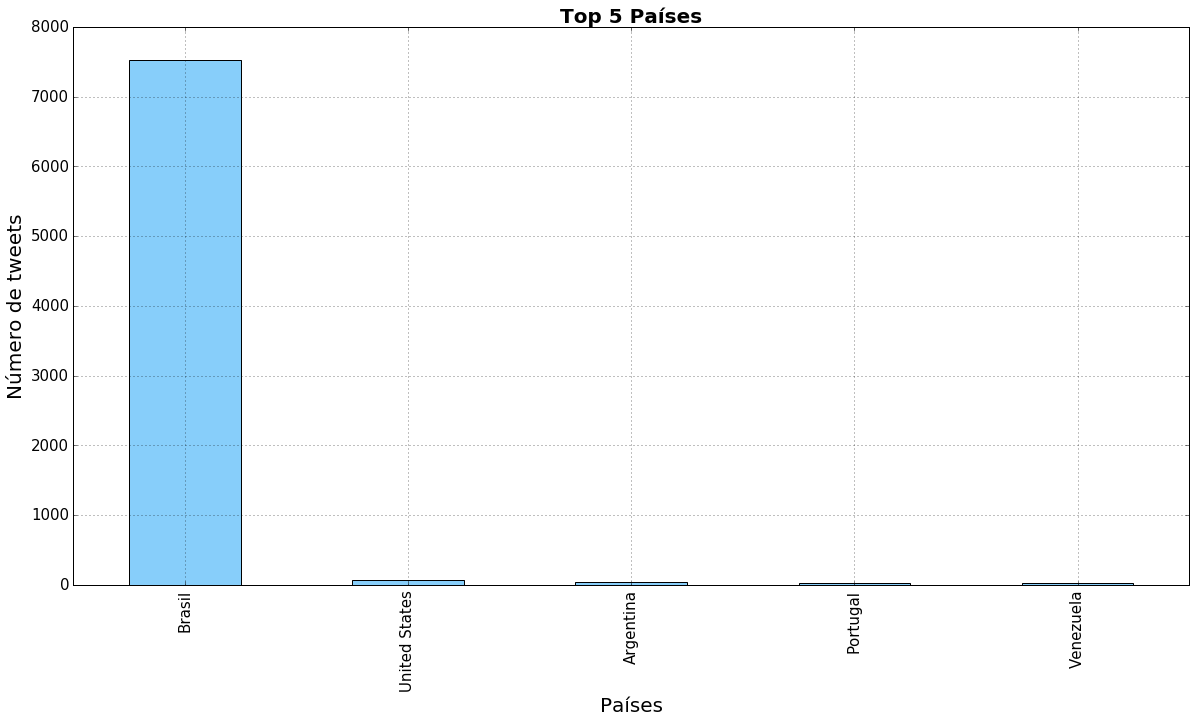
\includegraphics[width=1\textwidth]{Cap6/graficos/paises}}
	\vspace{-0.2cm}
	\caption{Países que mais realizaram \textit{tweets}}
	\fonte{Elaborado pelo autor}
	\label{paises}
\end{grafico}

Durante a votação no Congresso para a continuação do processo de Impeachment da Presidente Dilma Rousseff, os deputados declaravam o seu posicionamento dizendo se o seu voto era "SIM" \space para o processo ou "NÃO" \space caso o contrário.

O Gráfico~\ref{votacao}, apresenta a contabilização de palavras "SIM" \space e "NÃO" \space e as \textit{hashtags} \#ForaDilma e \#NaoVaiTerGolpe em \textit{tweets}. Dentro da \textit{hashtag} \#ForaDilma foi verificado a quantidades de palavras "SIM" \space isoladas e para a \textit{hashtag} \#NaoVaiTerGolpe verificou-se a disponibilidade da palavra "NÃO" \space . É válido informar que o Código~\ref{cod-vota} possui um filtro para não contabilizar as palavra "NÃO" \space que fazem parte da palavra-chave da \textit{hashtag} \#NaoVaiTerGolpe, podendo coletar apenas as palavras isoladas que fazem menções a votação.

\begin{grafico}[h]
	\centering
	\fbox{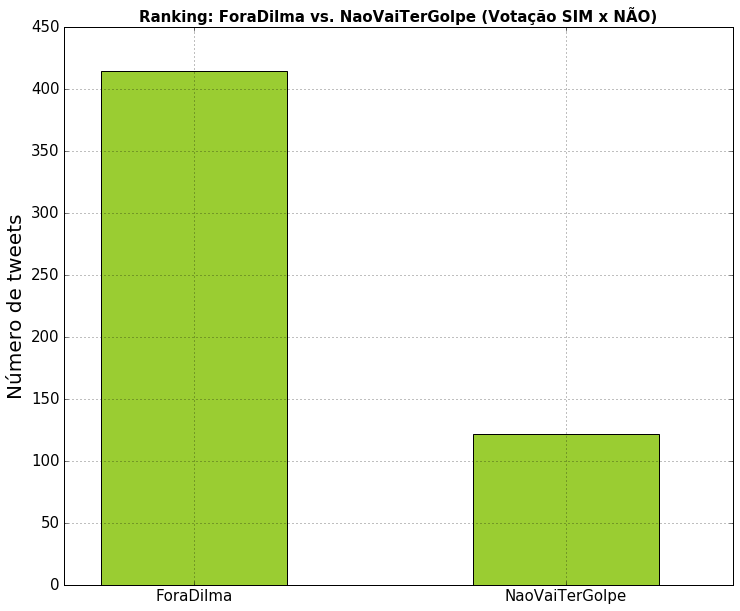
\includegraphics[width=1\textwidth]{Cap6/graficos/votacao}}
	\vspace{-0.2cm}
	\caption{Número de menções de "SIM" \space e "NÃO" \space em \textit{tweets}}
	\fonte{Elaborado pelo autor}
	\label{votacao}
\end{grafico}

Semelhante a solução anterior, é possível contabilizar as \textit{hashtags} e apresentá-las através do gráfico de setores, onde é possível verificar a porcentagem referente aos \textit{tweets} realizados com a \textit{hashtag} \#ImpeachmentDay, Gráfico~\ref{hashtag}. 

\begin{grafico}[h]
	\centering
	\fbox{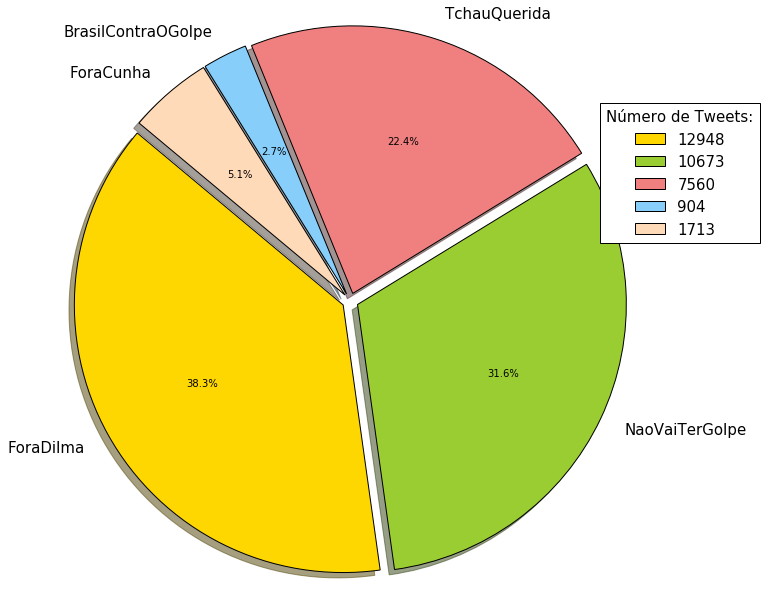
\includegraphics[width=1\textwidth]{Cap6/graficos/hashtag}}
	\vspace{-0.2cm}
	\caption{\textit{Hashtags} com o maior número de \textit{tweets}}
	\fonte{Elaborado pelo autor}
	\label{hashtag}
\end{grafico}

Nota-se no Gráfico~\ref{hashtag}, que as \textit{hashtags} \#ForaDilma e \#TchauQuerida somaram um total de 60,7\%, indicando que a maioria dos \textit{tweets} eram de apoio ao processo de Impeachment da Presidente da República, diferentemente dos 34,3\% dos \textit{tweets} que é o somatório de \#BrasilContraOGolpe e \#NaoVaiTerGolpe.

É possível também verificar na legenda o número de \textit{tweets} para cada uma das \textit{hashtags} apresentadas pelo gráfico. Nota-se que a \textit{hashtag} \#ImpeachmentDay não foi apresentada pois ela foi utilizada como critério de busca para a coleta destes dados, fazendo com que todos os \textit{tweets} possuam menções a essa \textit{hashtag}.

O Código~\ref{cod-fig-pol} explicado no capítulo anterior, constrói um gráfico em setores, onde é possível verificar a porcentagem de \textit{tweets} para nomes específicos, Gráfico~\ref{fig-pol}, porém não é possível, ainda, predizer se os argumentos a respeito destas pessoas são positivos ou negativos.

\begin{grafico}[h]
	\centering
	\fbox{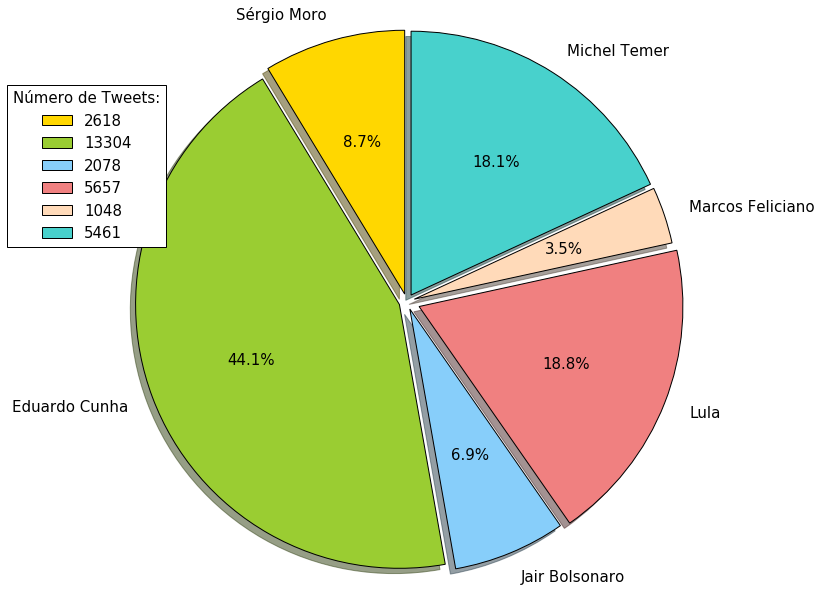
\includegraphics[width=1\textwidth]{Cap6/graficos/figuras-politicas}}
	\vspace{-0.2cm}
	\caption{Gráfico em setores para figuras importantes}
	\fonte{Elaborado pelo autor}
	\label{fig-pol}
\end{grafico}

O Gráfico~\ref{fig-pol}, demonstra que o nome mais mencionado foi de Eduardo Cunha e com apenas 2618 \textit{tweets} o nome de Michel Temer foi publicado. Até mesmo as menções ao ex-presidente Luiz Inácio "Lula" \space da Silva recebeu apenas 18,8\% do total dos nomes filtrados.

Semelhante ao Gráfico~\ref{hashtag}, é possível verificar o número de \textit{tweets} em que foi mencionado cada figura política. Porém não é contabilizado o nome de Dilma Rousseff, pois quase todos os \textit{tweets} fazem alguma menção a ela, resultando então em uma porcentagem mínima para os nomes apresentados no Gráfico~\ref{fig-pol}.

Uma outra maneira de apresentar a contabilização de palavras mais mencionadas é através da \textit{Word Cloud}. Conforme implementado e apresentado no Código~\ref{wordcloud} é possível visualizar algumas palavras-chaves, onde as mais citadas apresentam um tamanho de fonte maior, assim como as menos citadas são representadas através das palavras menores.

Através da Figura~\ref{fig:wordcloud}, é possível verificar claramente palavras como "ImpeachmentDay", "Dilma", "Cunha", "Brasil", "ForaDilma", "impeachment" dentre outras.

As cores disponibilizadas na Figura~\ref{fig:wordcloud} são da biblioteca padrão do \textit{Word Cloud} não representando nenhum outro indício a não ser uma funcionalidade aleatória para melhor visualizar as palavras.

\begin{figure}[h]
	\centering
	\fbox{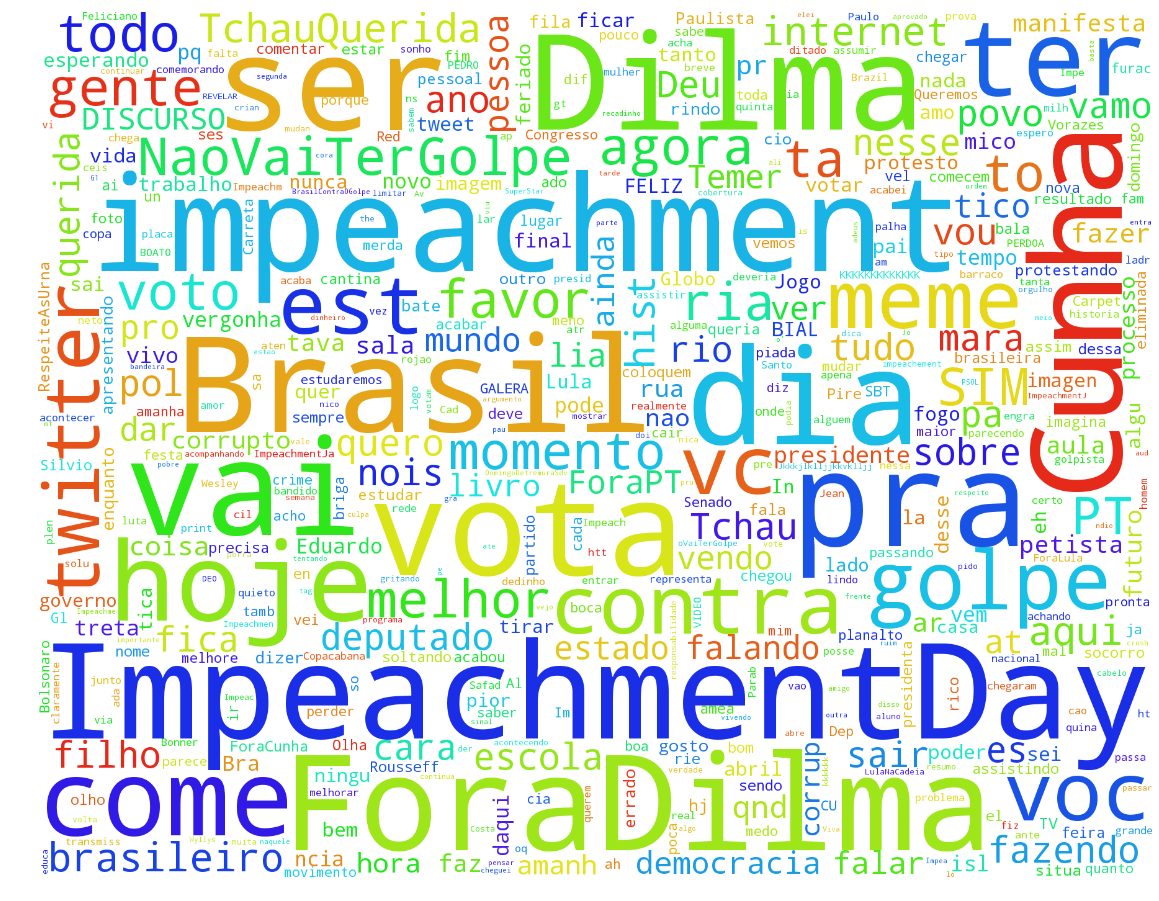
\includegraphics[width=1\textwidth]{Cap6/imagens/wordcloud}}
    \vspace{-0.2cm}
	\caption{\textit{Word Cloud} das 500 palavras mais mencionadas}
	\fonte{Elaborado pelo autor}
	\label{fig:wordcloud}
\end{figure}

A biblioteca \textit{Word Cloud} na linguagem Python, permite que o desenvolvedor utilize alguma imagem como modelo. Onde as cores e o posicionamento das palavras são disponibilizados na tentativa de representar a imagem modelo.

A Figura~\ref{fig:worddilma} ilustra este tipo de funcionalidade apresentando a imagem modelo uma foto da Presidente suspensa Dilma Rousseff. Ao lado direito é demonstrado o \textit{Word Cloud} gerado, que representa cores com tonalidades semelhantes a imagem modelo.

Da mesma maneira que a Figura~\ref{fig:wordcloud} apresenta as palavras com mais menções, o \textit{Word Cloud} da Figura~\ref{fig:worddilma} também disponibiliza as 500 palavras e \textit{hastags} mais publicadas coletadas durante o dia da votação no Congresso brasileiro.

\begin{figure}[h]
	\centering
	\fbox{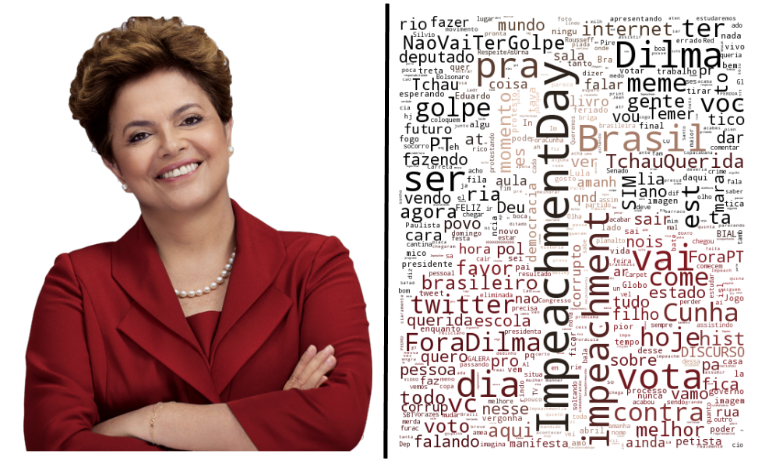
\includegraphics[width=1\textwidth]{Cap6/imagens/worddilma}}
	\vspace{-0.2cm}
	\caption{\textit{Word Cloud} utilizando imagem como modelo}
	\fonte{Elaborado pelo autor}
	\label{fig:worddilma}
\end{figure}

Exercendo o uso dos atributos de coordenadas, implementados no Código~\ref{mapa} utilizando a biblioteca \textit{Folium}, é possível verificar a distribuição dos \textit{tweets} geograficamente. As informações de latitude e longitude permitem que cada \textit{tweet} seja representado por um marcador conforme ilustrado pela Figura~\ref{fig:mapa}.

A coleta de dados resultou em um arquivo JSON com 358.293 \textit{tweets}, porém apenas 470 destas publicações possuem informações de coordenadas. Este total de \textit{tweets} com atributos de posições geográficas representa apenas míseros 0,13\% da totalidade dos dados, não sendo possível, então, afirmar que é um padrão ou uma tendência.

A utilização dos dados geográficos, representados pela Figura~\ref{fig:mapa}, demonstra mais um das funcionalidades que as bibliotecas da linguagem Python disponibiliza para a apresentação dos dados. Através do \textit{IPython} é possível navegar através do mapa, ter interações com os marcadores e se distanciar ou aproximar para verificar detalhes sobre as localidades da publicação.

\begin{figure}[h]
	\centering
	\fbox{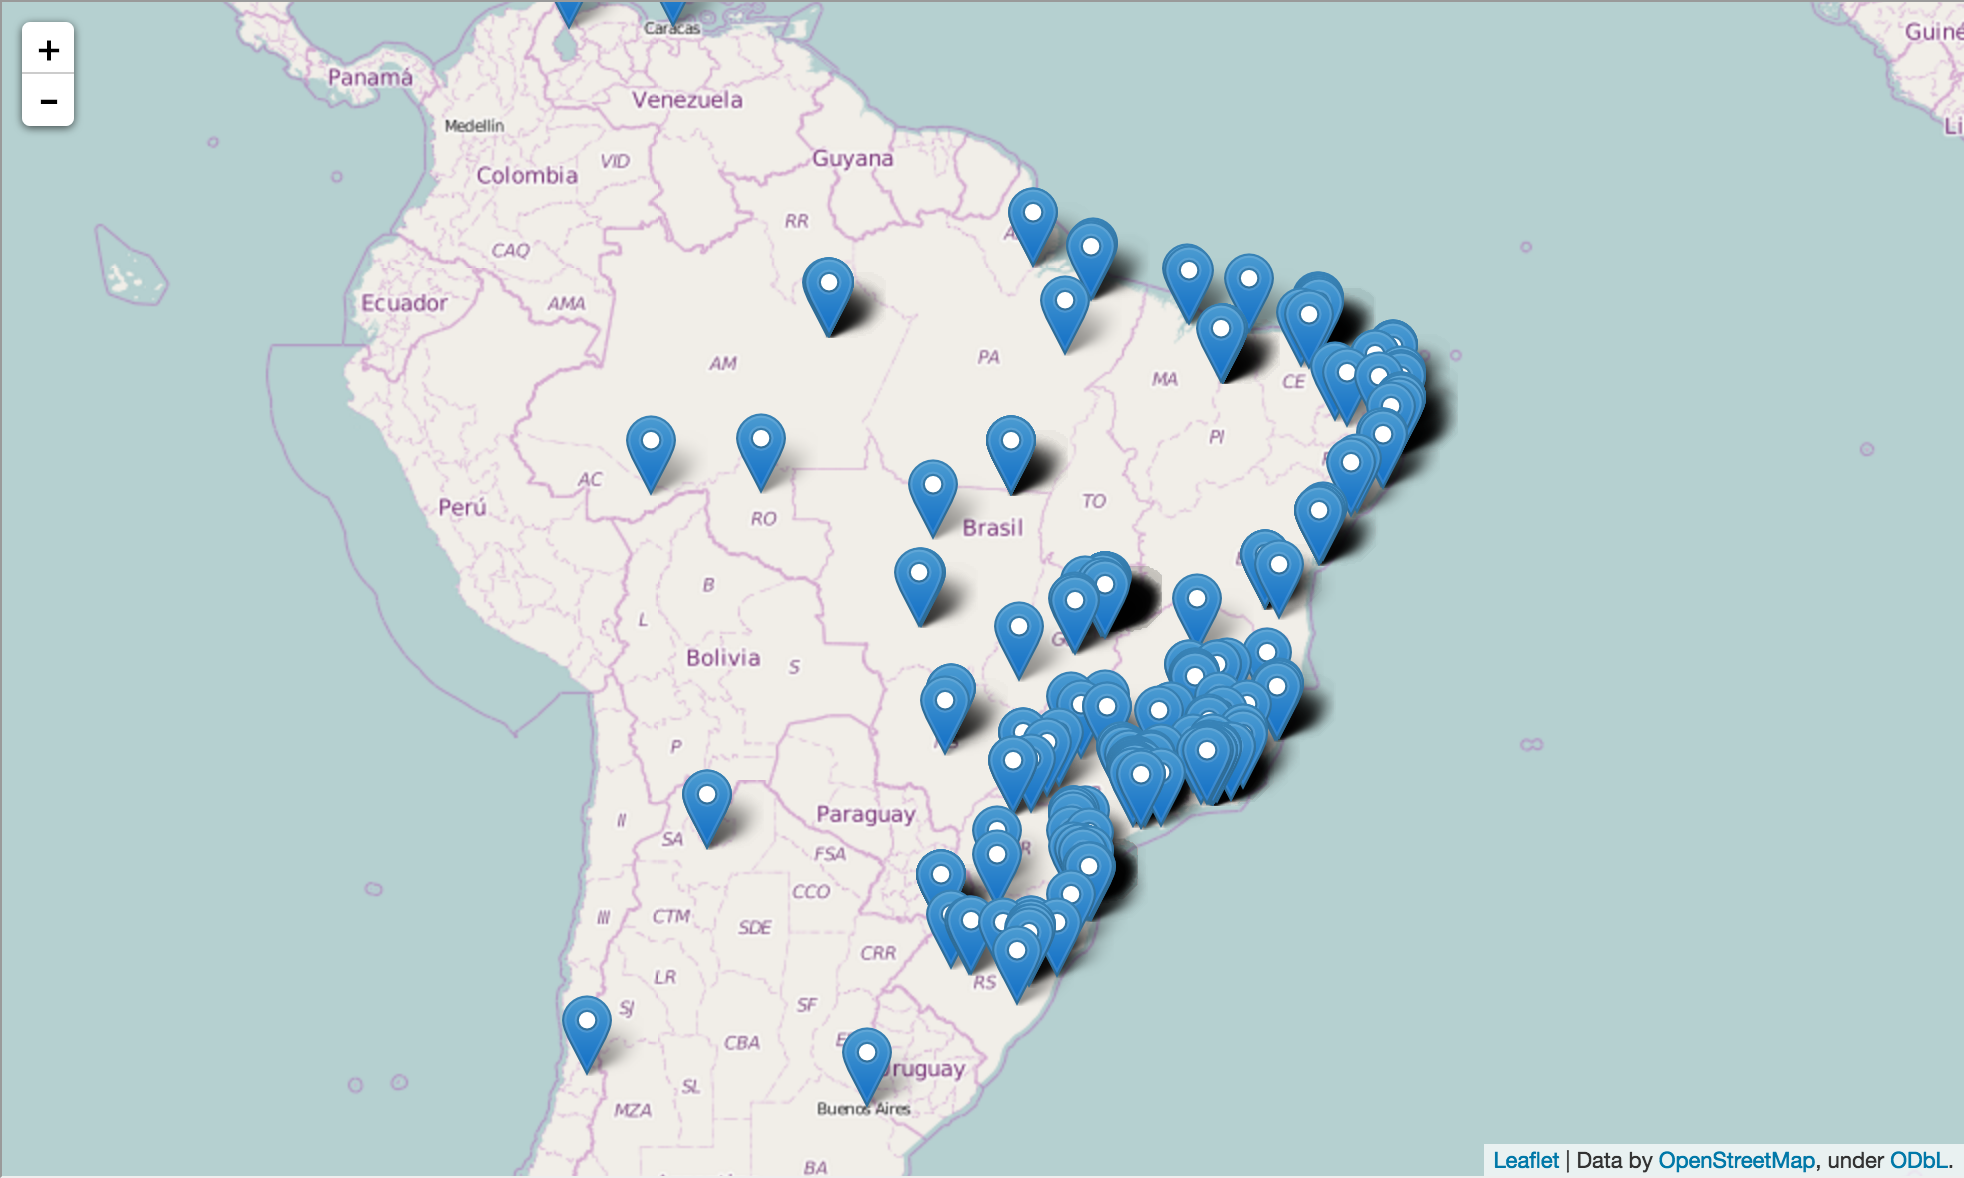
\includegraphics[width=1\textwidth]{Cap6/imagens/mapa}}
	\vspace{-0.2cm}
	\caption{Distribuição geográfica de \textit{tweets}}
	\fonte{Elaborado pelo autor}
	\label{fig:mapa}
\end{figure}

\begin{grafico}[h!]
	\centering
	\fbox{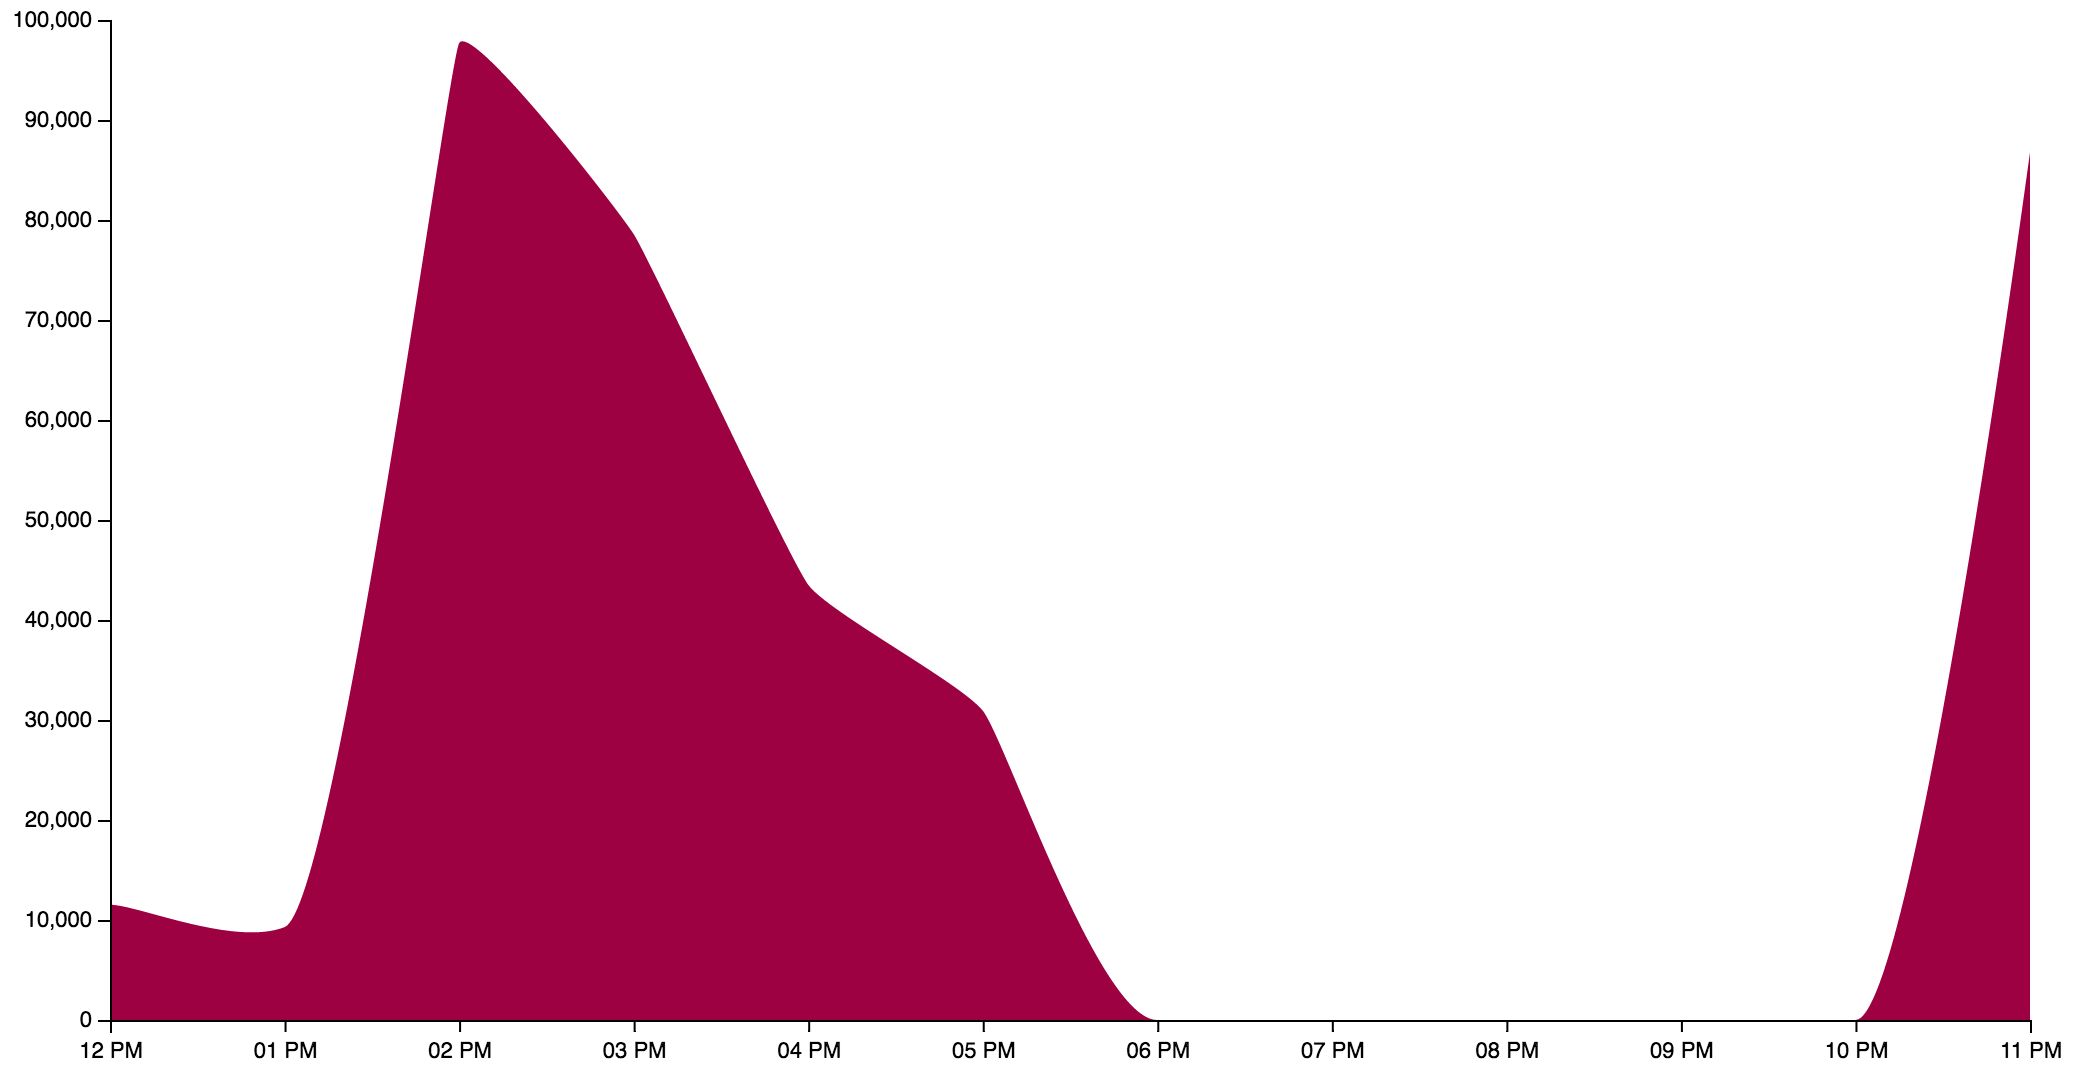
\includegraphics[width=1\textwidth]{Cap6/graficos/time}}
	\vspace{-0.2cm}
	\caption{Publicação de \textit{tweets} por hora}
	\fonte{Elaborado pelo autor}
	\label{time}
\end{grafico}

O Gráfico~\ref{time} apresenta a quantidade de publicações de \textit{tweets} por hora dentro das 12 horas de coletas.

É notado que no período das 14 horas (02 PM) ocorreu o maior número de \textit{tweets}, chegando a quase 100 mil publicações. O horário da votação no congresso começou às 16 horas, horário de Brasília, momento em que teve as maiores baixas apresentas pelo Gráfico~\ref{time}. A ascensão dos \textit{tweest} volta acontecer após às 22 horas, próximo ao horário de conclusão e resultado da votação.

As bibliotecas que Python dispõe, permitiu a apresentação de gráficos em colunas, setores e áreas. Também a visualização de palavras mais mencionadas através do \textit{Word Cloud} e a distribuições dos \textit{tweest} através de coordenadas para ser apresentadas em mapa.







